\chapter{Calibration Strategy}
\label{ch:exec-summ-calib}

%%%%%%%%%%%%%%%%%%%%%%%%%%%%%%%%%%%%%%%%%%%%%%%%%%%%%%%%%%%%%%%%%%%%
%%%%%%%%%%%%%%%%%%%%%%%%%%%%%%%%%%%%%%%%%%%%%%%%%%%%%%%%%%%%%%%%%%%%
\section{Introduction}
\label{sec:calibintro} %% 2 pages


The DUNE \dword{fd} presents a unique challenge for calibration in many ways. Not only because of its size---the largest \dword{lartpc} ever constructed -- but also because of its depth. It differs both from existing long-baseline neutrino detectors, and existing \dwords{lartpc}. Also, the deep underground location results in low cosmic ray rates limiting the usage of it as a calibration source. Another important difference is that DUNE does not as yet have a near detector design and, unlike MINOS and \dword{nova}, the near detector is unlikely to be very much like the \dword{fd}.

Like any \dword{lartpc}, DUNE has as a great advantage precision tracking and ultra-clean target medium, but, to fully exploit this will require significant challenges in understanding its detector response. This challenge is driven by the inherently highly convolved detector response model and strong correlations that exist between various calibration quantities. For example, the
drift vertex of a track, the drift distance, the initial time the track occurs ($t_0$) and the drift velocity are all highly correlated. In turn, the drift velocity depends on the electric field. The electric field itself may have local variations in space or in time for an enormous detector operating for multiple decades.
The determination of energy associated to an event of interest will depend on the simulation model, associated parameters, non-trivial correlations between the parameters and spatial and temporal dependence of those parameters. These variations in parameters occur since the detector is not static. Changes can be abrupt (e.g. noise, a broken resistor in the field cage), or ongoing (e.g. exchange of fluid through volume, ion accumulation). Unfortunately, the relevant calibration sampling timescales of such changes are not currently known, though ongoing and past experiments may be able to place reasonable limits on how often events may occur.

A convincing measurement of CP violation, or a resolution of the neutrino mass ordering, will require a demonstration that the overall detector response is well understood, and can be extrapolated across the entire physics regions of interest.
This document will describe a strategy for detector calibration for both 
\dwords{spmod} and \dwords{dpmod}
using dedicated \dword{fd} systems and/or existing calibration sources. A large portion of the calibration work reported here is done under the joint  \dword{sp} and \dword{dp} Calibration task force (TF) group formed in Fall 2017. Calibration sources and systems provide measurements of the detector response model parameters, or provide tests of the response model.
Figure~\ref{fig:calibneeds} shows the broad range of categories of measurements calibrations can provide. In addition to this, calibration measurements also provide corrections applied to data, data-driven efficiencies, systematics and particle responses. Figure~\ref{fig:calibneeds} also lists some of the critical calibration parameters for DUNE's detector response model for either  \dword{sp} or \dword{dp}.
Due to the significant interdependencies of many parameters (recombination, drift velocity, electric field), a calibration strategy will either need to iteratively measure parameters, and/or find sources which break these correlations. 

\begin{dunefigure}[Categories of measurements provided by Calibration.]{fig:calibneeds}{Categories of measurements provided by Calibration.}
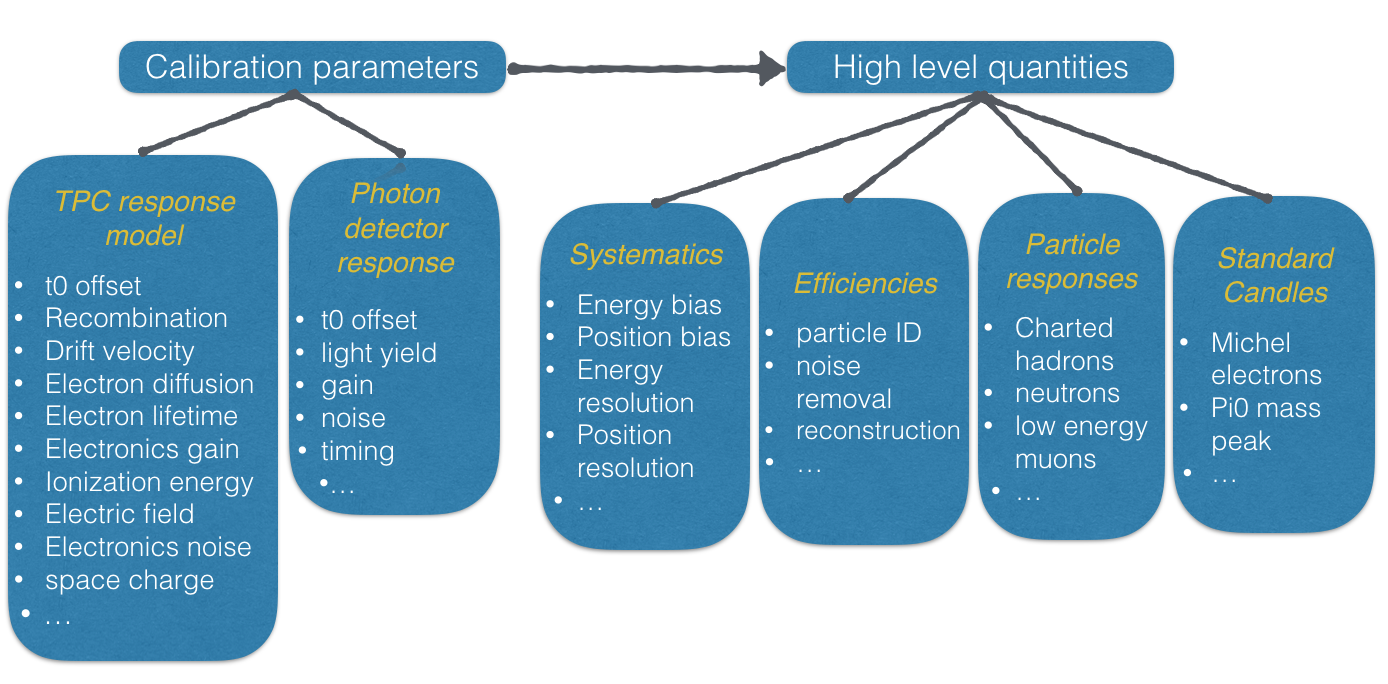
\includegraphics[width=.9\textwidth]{calib-needs.png}
\end{dunefigure}

The systematic uncertainties on high level physics quantities drive how precisely each parameter need to be measured. For example, how precisely will the drift velocity need to be measured to know fiducial volume better than \num{1}\%?  What does \num{1}\% energy bias mean for electron drift-lifetime and electronics calibration measurements? Section~\ref{sec:calibphys} describes the physics requirements for calibration for long-baseline, supernovae and other physics such as nucleon decay and exotic searches. In general, the calibration program must provide measurements at the few percent or better level, and must also provide sufficient redundancy in the measurement program.


Section~\ref{sec:extcalib} describes calibration measurements from 
other \dword{lar} experiments that are of relevant for DUNE. This includes both past measurements (e.g., ArgoNeuT, DUNE \dword{35t}, \dword{microboone}, LArIAT), anticipated measurements from ongoing and future experiments (e.g., \dword{microboone}, \dword{protodune}) as well as from small scale \dword{lartpc} test stands. Some parameters, like the argon ionization energy, are believed to be universal and have been measured ex-situ. \Dword{protodune} and previous measurements provide independent, critical tests of the response model, where the choice of parameterization and values correctly reproduces real detector data. However informative, not all of the previous ex-situ measurements will be directly extrapolatable to DUNE.

Section~\ref{sec:existsource} describes existing calibration sources, their limitations and remaining studies necessary for the TDR. Existing calibration sources include (beam or atmospheric)  neutrino-induced samples, cosmic rays, argon isotopes and instrumentation devices such as liquid argon purity monitors, temperature and current monitors. For example, drift velocity depends on temperature (and electric field), so measurements of temperature reduce the interdependencies in understanding drift velocity. While there are many existing calibration sources, each source comes with its own challenges. We further distinguish between sources which are used to measure a response model parameter, and measurements which test the response model. For example, electrons from 
%pion or (SG: do we understand the spectrum from pion days as we understand Michel; unsure, comment out for now.
muon decay (Michel electrons) are very useful to study the detector response to low energy electrons ($\sim$ \SI{50}{\MeV}). However, low-energy electrons have major reconstruction challenges due to the loss of charge from radiative photons as demonstrated in \dword{microboone}~\cite{uBmichel}. In terms of source category, Michel electrons are considered as an important, independent, and necessary test of the TPC energy response model, and not as a measurement of a particular response parameter.

Section~\ref{sec:DP} describes some specific calibration-related considerations for \dword{dp}. One of the biggest challenges for \dword{dp} is the \SI{12}{\m} long single drift path and ion accumulation at the liquid-gas interface.

Section~\ref{sec:extsystems} describes dedicated external calibration systems currently under consideration for DUNE to perform calibrations that cannot be achieved fully from existing sources or external measurements. For each system considered, a reference design is described along with motivation, possible measurements and remaining studies for the TDR. All the systems proposed are currently being actively discussed in the Calibration Task Force and were agreed as critical systems by the DUNE collaboration. While the proposed external calibration systems are being finalized, the calibration TF focused on finalizing the feedthrough penetration design for the \dword{spmod} and made necessary accommodations for calibration systems. The current cryostat penetration design for \dword{spmod} calibrations is described in Section~\ref{sec:FTs}. The TF will soon start focusing on \dword{dpmod} design and accommodations in terms of calibration penetrations. Under current assumptions, the calibration strategy and proposed calibration systems described in this document are applicable to both \dwords{sp} and \dwords{dp}. 

Section~\ref{sec:calibsum} provides a summary of the document along with future steps for calibration and a path to TDR. 
%Any specific differences with \dword{sp} and additional considerations for  \dword{dp}  are interspersed through out the document where necessary.
 
    